\section{PX4 SITL simulation and validation}
\label{sec:test-2-sitl}

Section \ref{sec:devenv} describes the software-in-the-loop simulation mode developed by PX4.
Using this mode makes it possible to test and validate the correct operation of each part in the program's architecture.
To start, it is necessary to validate that it is possible to use the connection between the simulated flight controller and the DroneVisionControl program to send commands to the simulated vehicle, as well as to capture images from a connected camera and use them to test the detection algorithm.
The full list of validation steps is, therefore:
\begin{enumerate}
    \item Verify that it is possible to start the simulated flight controller and that it connects to the 3D simulator vehicle.
    \item Connect the DroneVisionControl program to the flight controller and send basic commands.
    \item Retrieve images from a camera and run computer vision detection on them.
    \item Integrate the last three steps by running the hand-gesture control solution described in section \ref{sec:hands}
\end{enumerate}

For this purpose and to be able to run with a minimal configuration, the Gazebo simulator\footnote{\url{https://gazebosim.org/home}} included with the base PX4 installation will be used as the 3D environment.
This simulator works inside Linux on the same computer that runs the SITL PX4.
To be able to later transition into using the AirSim simulator instead, which runs in Windows, with minimal changes, for this test, PX4, Gazebo and the DroneVisionControl program will run inside the Windows Subsystem for Linux.
The complete installation process necessary to run these tests is explained in appendix \ref{app:install-dev-env} and \ref{app:install-dronecontrol-rpi}.

\begin{figure}
  \centering
  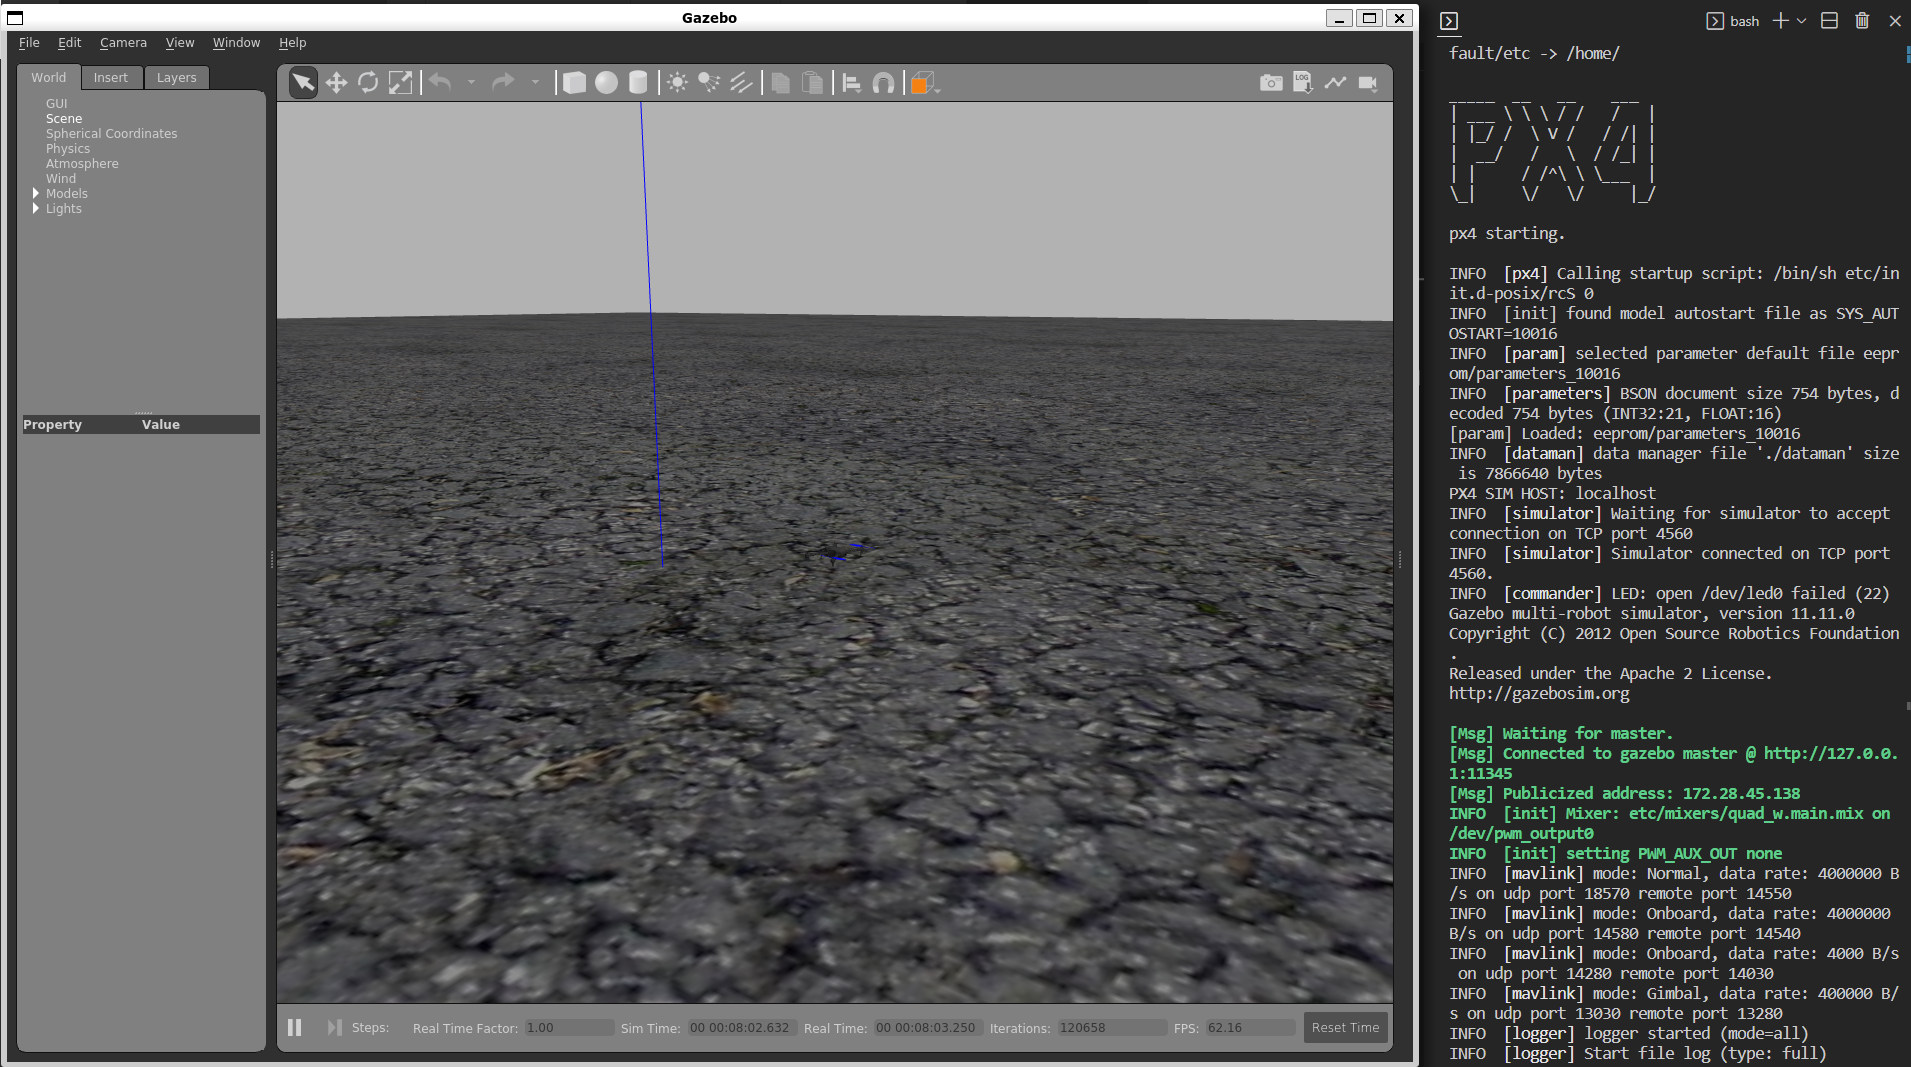
\includegraphics[width=\textwidth, keepaspectratio]{img/gazebo.png}
  \caption{Gazebo simulator (left) and output from the PX4 terminal (right) after PX4's software-in-the-loop mode is started}\label{fig:gazebo}
\end{figure}

Once both parts are installed, PX4 and Gazebo can be started by running the \texttt{make\ px4\_sitl\ gazebo} command inside its installation folder.
The result of this command can be seen in figure \ref{fig:gazebo}, where the left part shows the user interface and 3D world of the Gazebo simulator and the right side contains the PX4 console that can be used for sending commands and changing the configuration parameters of the simulated flight controller.
The most straightforward command to test is takeoff, which is done by sending \texttt{commander takeoff} through the console.
Figure \ref{fig:gazebo-takeoff} shows the simulator's state after the takeoff command, where the vehicle model has climbed to the default height of 2.5 meters above the ground.
The command to land the vehicle again is \texttt{commander land}.

\begin{figure}
  \centering
  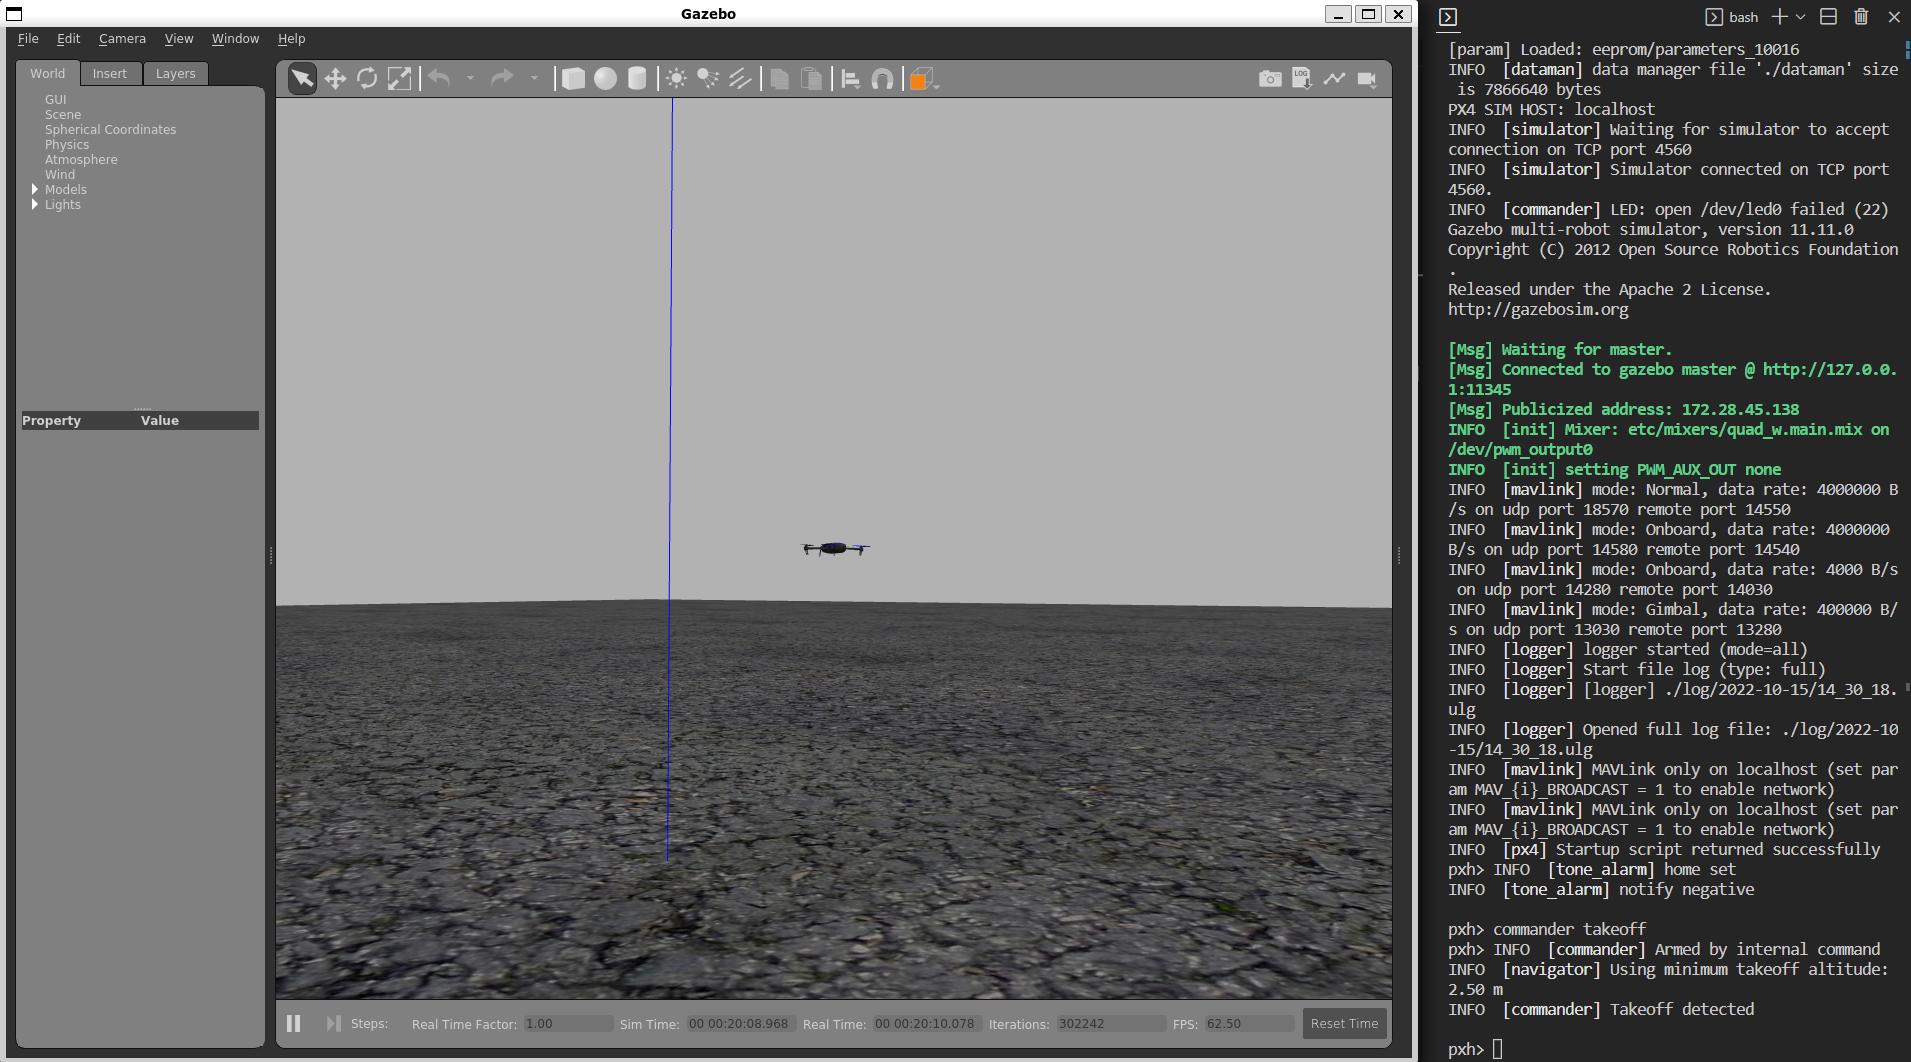
\includegraphics[width=\textwidth, keepaspectratio]{img/gazebo-takeoff.png}
  \caption{Gazebo simulator (left) and output from the PX4 terminal (right) after the takeoff command has been executed}\label{fig:gazebo-takeoff}
\end{figure}

The next step is to connect the DroneVisionControl application.
The camera testing tool described in section \ref{subsec:cam-tool} has been developed specifically for this test so that it is possible to establish a connection to PX4 SITL and process images without engaging any of the program's control modules.
The commands are then sent to PX4 through keyboard input.
For example, the key "T" will make the simulated vehicle take off.
Figure \ref{fig:sitl-hand} shows the image and text output of the program when the test camera tool is run with the hand detection feature activated.
On the left side, the detection algorithm tracks the joint of the hand present in the captured image and on the right side, the logged information shows when the connection is established and keyboard commands are sent to the simulator.


\begin{figure}
  \centering
  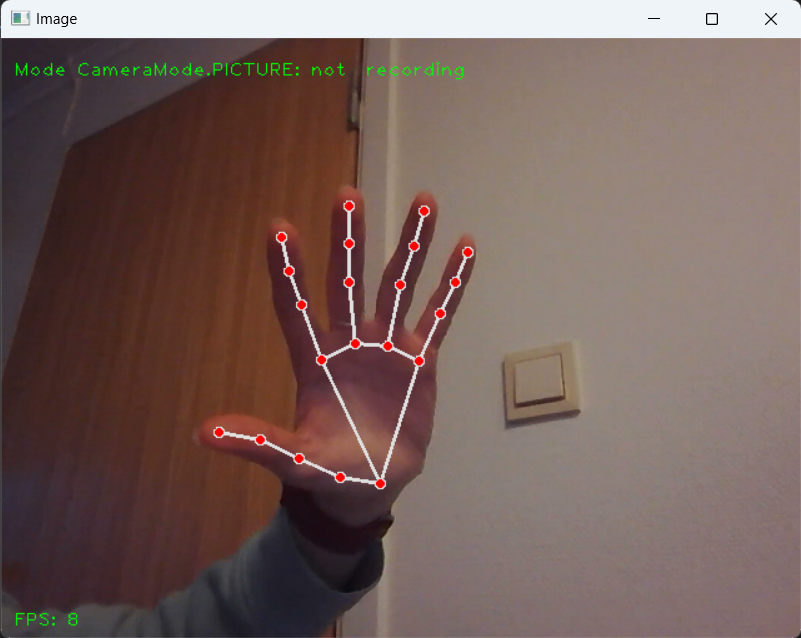
\includegraphics[width=\textwidth, keepaspectratio]{img/sitl-hand.png}
  \caption{Hand detection algorithm running on images taken from the computer integrated webcam}\label{fig:sitl-hand}
\end{figure}

The entire execution of a test of the hand-gesture-based control solution is shown in this \href{https://l-gonz.github.io/tfg-giaa-dronecontrol/videos/test-sitl-hand}{video}\footnote{\url{https://l-gonz.github.io/tfg-giaa-dronecontrol/videos/test-sitl-hand}} in this link and an image extracted from it can be seen in figure \ref{fig:sitl-hand-video}.

\begin{figure}
  \centering
  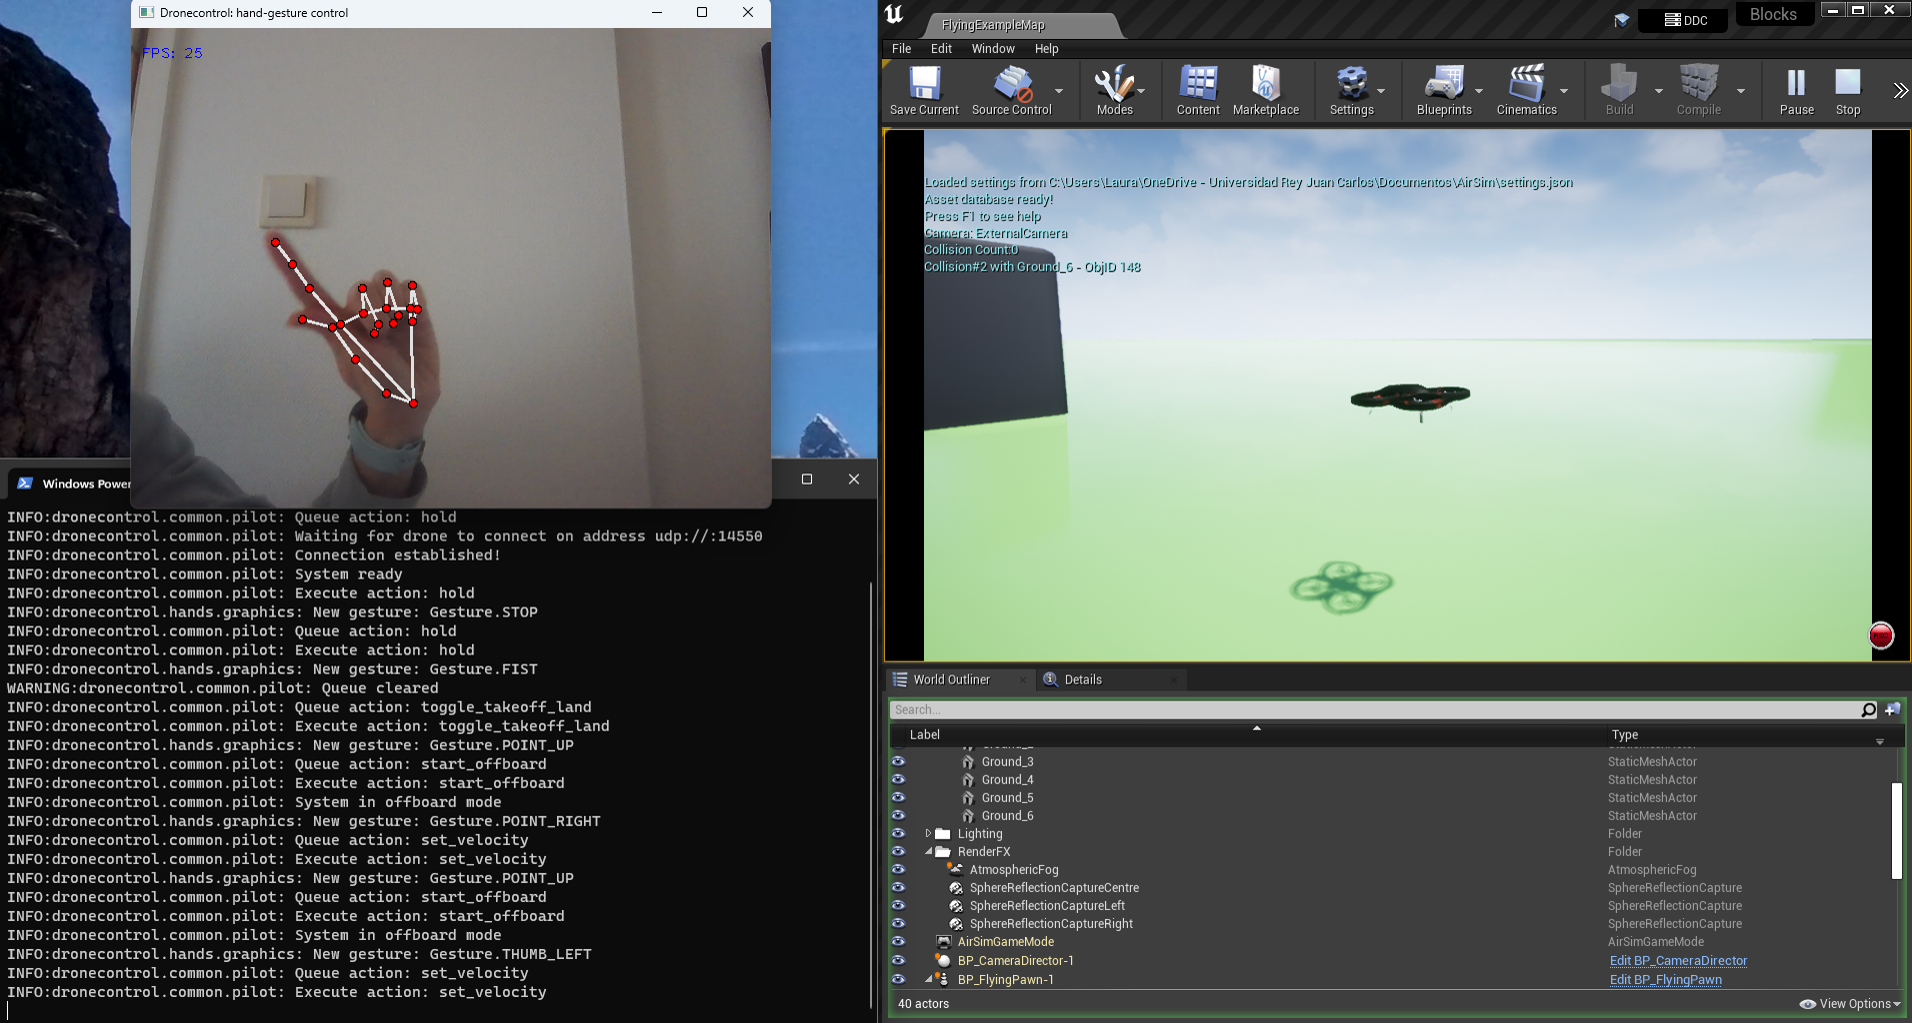
\includegraphics[width=\textwidth, keepaspectratio]{img/video-hand-sitl.png}
  \caption{Single frame from the video showing the full execution of the hand-gesture control solution}
  \label{fig:sitl-hand-video}
\end{figure}


\subsection{PX4 SITL validation with AirSim}
\label{sec:test-3-airsim}

The end goal for the testing environment is for it to use the AirSim simulator to take advantage of its 3D-world and computer vision capabilities.
For this reason, it becomes necessary to validate that the new simulator can run correctly on Unreal Engine on the computer and interact with PX4 as well as it did with the default Gazebo simulator and that all the necessary features for detection, tracking and following work as expected.
All these characteristics will be checked in the order below:
\begin{enumerate}
    \item Verify that the AirSim simulator can start, connect to the PX4 SITL through the WSL virtual network and receive commands from the PX4 terminal.
    \item Check that the DroneVisionControl program can connect to both AirSim through the WSL network to receive images and PX4 through the local network to send movement commands.
    \item Test the pose recognition algorithms on the images obtained from the AirSim simulation.
    \item Check that the follow solution can control the vehicle's velocity directly in PX4's offboard mode.
\end{enumerate}

In the first place, the AirSim simulator needs to be installed in the Windows host.
The complete installation process is described in appendix \ref{app:install-dev-env}.
There are specific configuration parameters that have to be set to be able to connect the AirSim simulator in Windows to the PX4 SITL running inside WSL.
On the simulator side, AirSim's settings file has to include a line defining the IP address of the network interface to use.
This parameter, along with the entire configuration file used for SITL testing, can be found in appendix \ref{app:airsim-config}.
On the PX4 side, it is necessary to specify that the simulator will attach through a different IP address than \texttt{localhost}.
This is done by setting the \texttt{PX4\_SIM\_HOST\_ADDR} environment variable in the Linux system to the IP address of the Windows host on the WSL virtual network before starting PX4 as follows:
\begin{minted}{bash}
export PX4_SIM_HOST_ADDR=[IP-address]
make px4_sitl none_iris
\end{minted}
This starts the software-in-the-loop execution, which attempts to attach to an already running simulator listening on the IP address specified and the TCP port 4560, in this case, AirSim.
Therefore, every time either PX4 or AirSim stops its execution, both of them have to be restarted in the specific order of first the AirSim simulator and then the PX4 flight controller.
Figure \ref{fig:airsim-sitl} shows the testing environment after the AirSim simulator and the PX4 console have been started successfully.

\begin{figure}
  \centering
  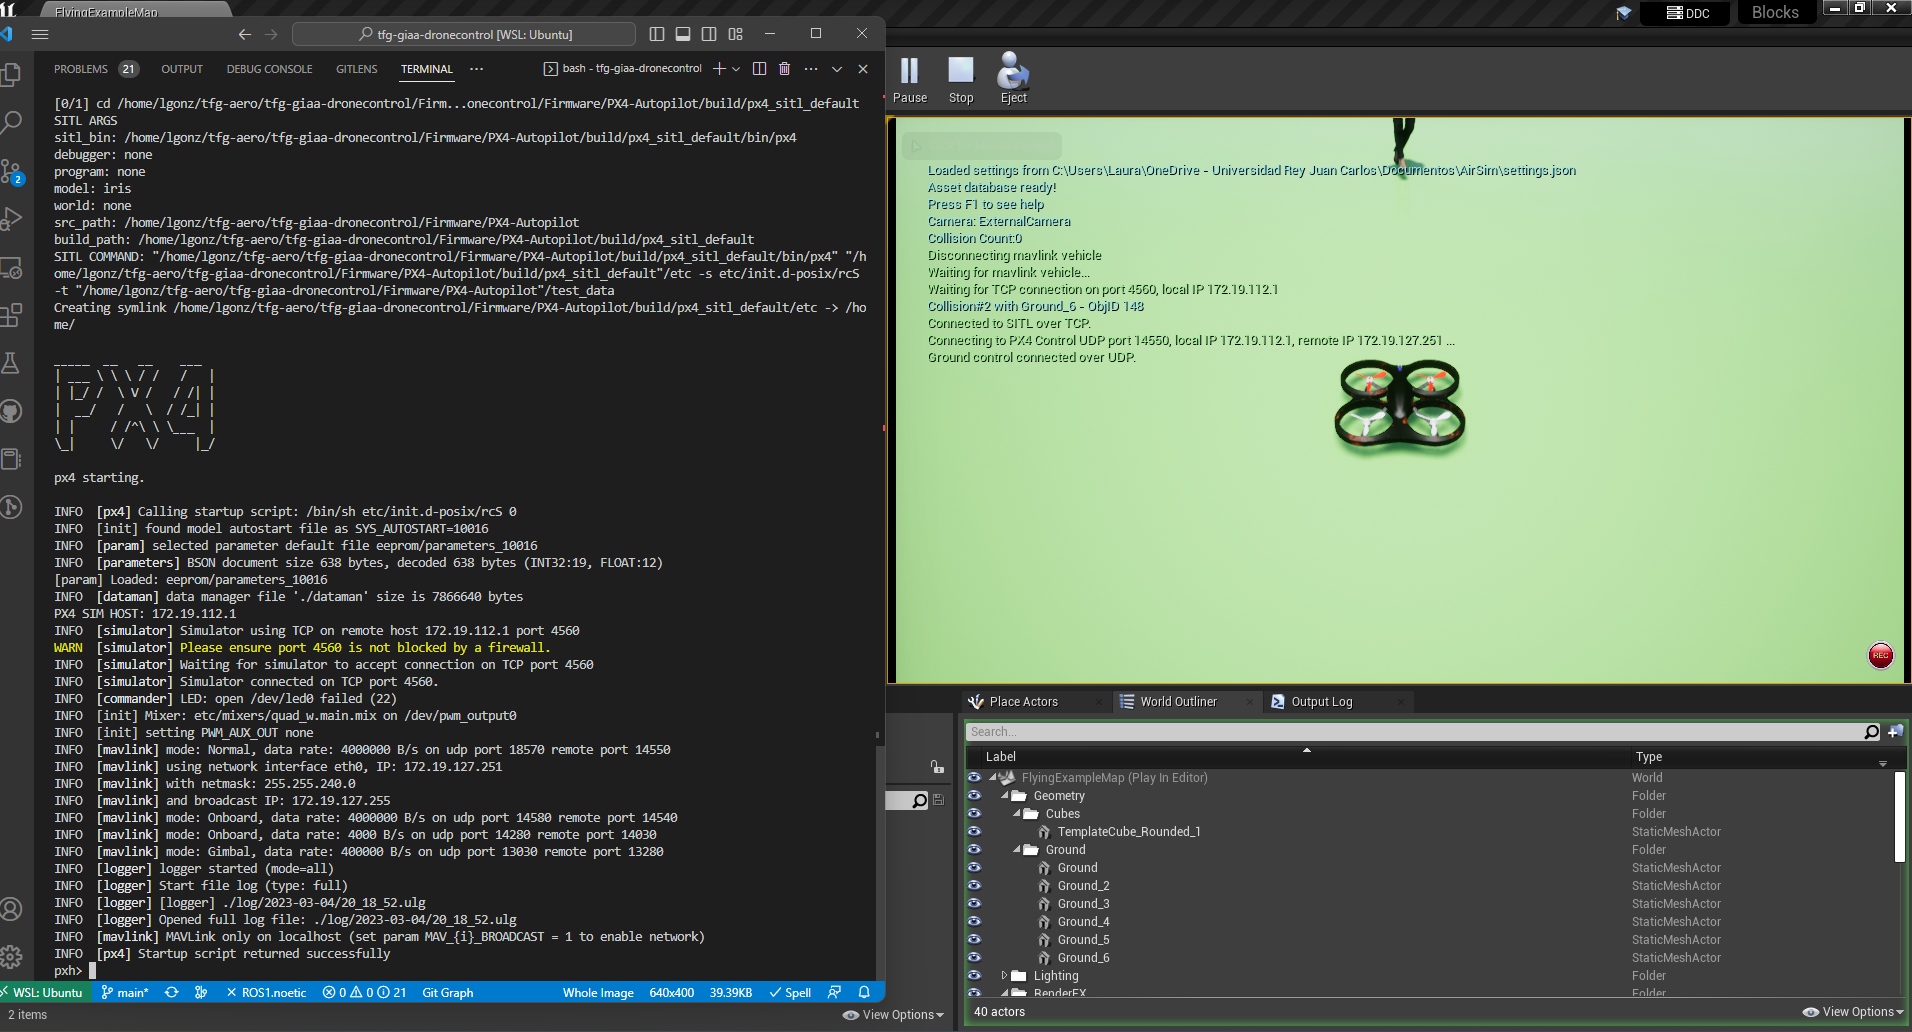
\includegraphics[width=\textwidth, keepaspectratio]{img/airsim-sitl.png}
  \caption{AirSim environment connected to PX4 flight stack running in SITL mode}
  \label{fig:airsim-sitl}
\end{figure}

At this point, it is possible to use the PX4 console to send takeoff and land commands to the simulator and observe the 3D model of the vehicle climb into the air.
To test the detection and tracking of human figures from images taken inside the simulator, one can again use the camera testing tool provided with DroneVisionControl.
Figure \ref{fig:airsim-sitl-pose} shows the output when the tool is run with a 3D model of a person situated in front of the drone in the simulated world and the command:
\mint{bash}{dronevisioncontrol tools test-camera --wsl --sim --pose-detection}
In the image, the computer vision utility detects the main features of the human body and a bounding box is drawn around it.
Meanwhile, the logged output from the program shows two calculated positions in the terminal: the x coordinate of the midpoint of the bounding box and the percentage of the image height covered by the height of the bounding box.
These two numbers are the inputs for the PID controllers used in the follow solution as described in section \ref{sec:follow} so that the output can be used to calibrate the distance from which the drone is to follow the person when that control mode is engaged.

\begin{figure}
  \centering
  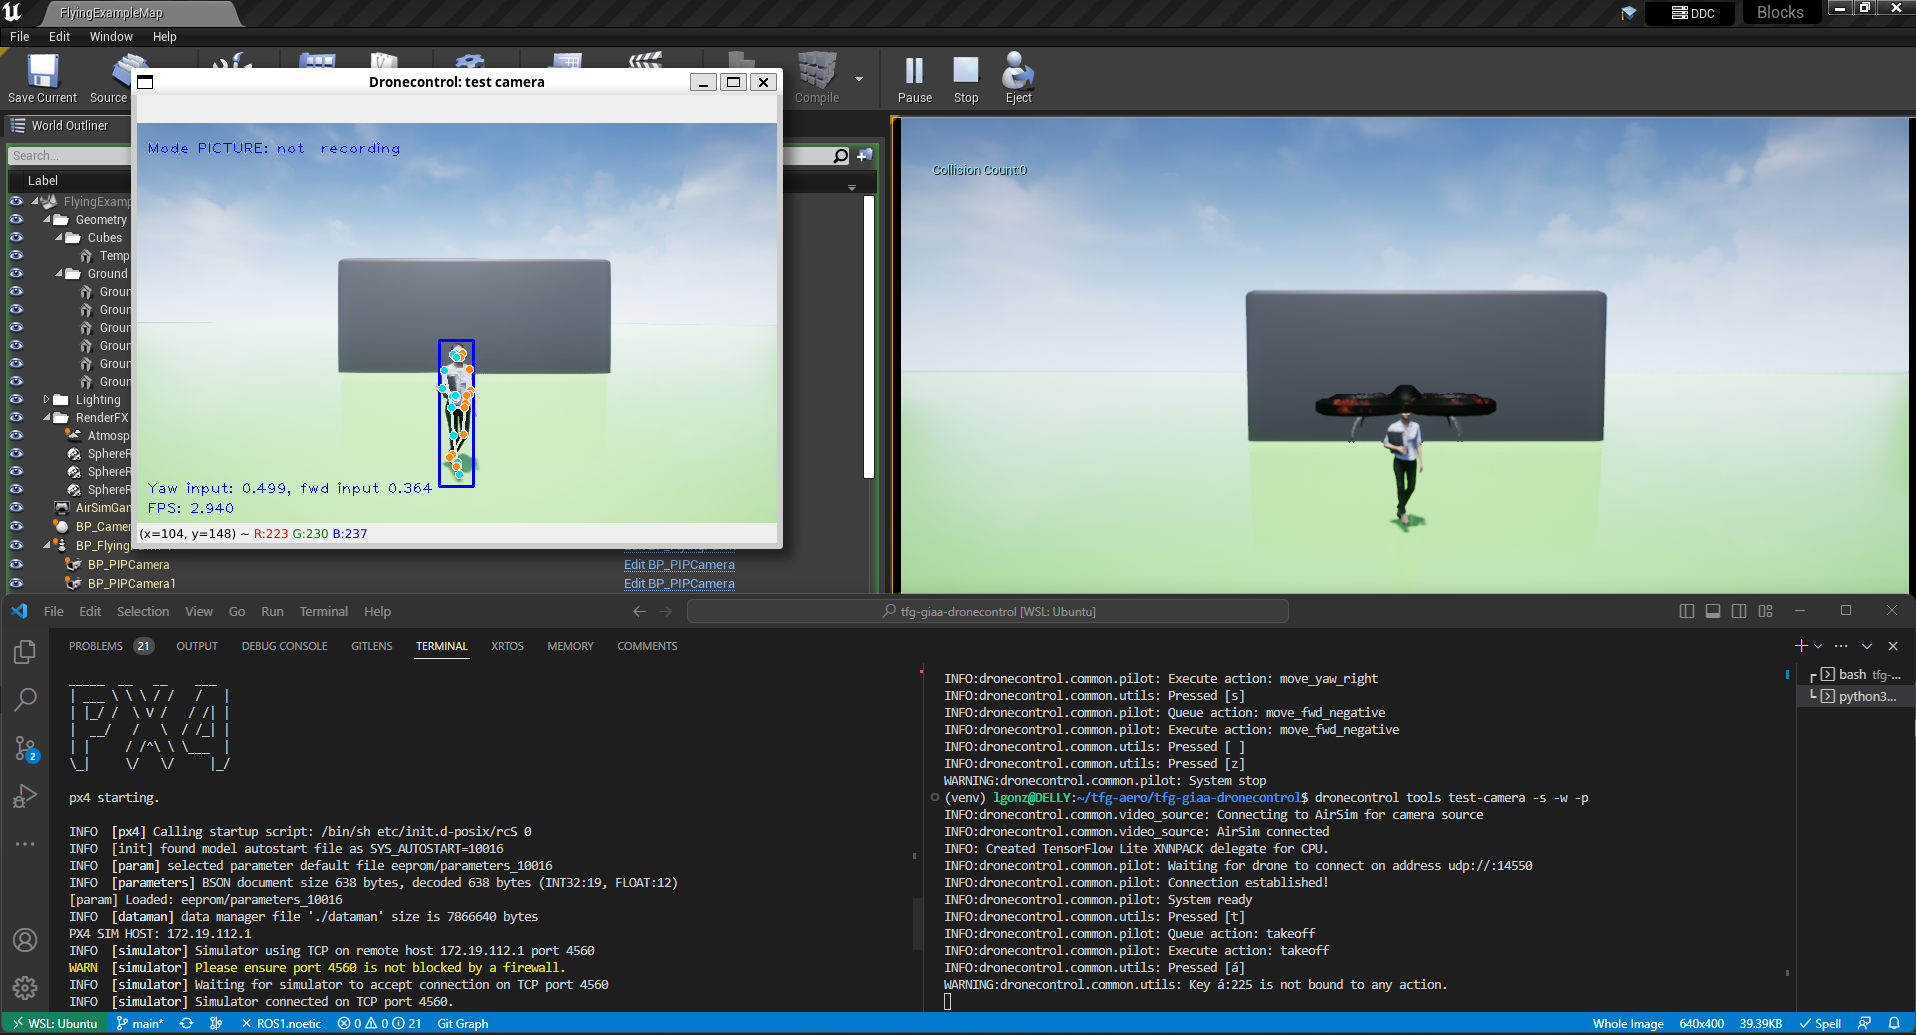
\includegraphics[width=\textwidth, keepaspectratio]{img/airsim-sitl-pose.png}
  \caption{AirSim, PX4 and DroneVisionControl applications running side-by-side and connecting to each other}
  \label{fig:airsim-sitl-pose}
\end{figure}

Now that the testing environment is working as expected and before it is used to tune the PID controllers in the follow solution to the response of the vehicle's movement in the next section, it is possible to verify that the controllers are capable of reacting to changes in the position of the figure by only enabling their proportional term with an appropriately low magnitude to keep the movement slow and smooth.
The drone movement when running the follow control program with values of 10 and 2 on the proportional term of the yaw and forward controllers, respectively, which can be done with the command \mintinline{bash}{dronevisioncontrol follow --sim --yaw-pid (10, 0, 0) --fwd-pid (2, 0, 0)}, is shown in this \href{https://l-gonz.github.io/tfg-giaa-dronecontrol/videos/test-sitl-follow}{video}\footnote{\url{https://l-gonz.github.io/tfg-giaa-dronecontrol/videos/test-sitl-follow}} and a frame extracted from it can be seen in figure \ref{fig:airsim-test-follow}.
\todo[inline]{Match text to video}

\begin{figure}
  \centering
  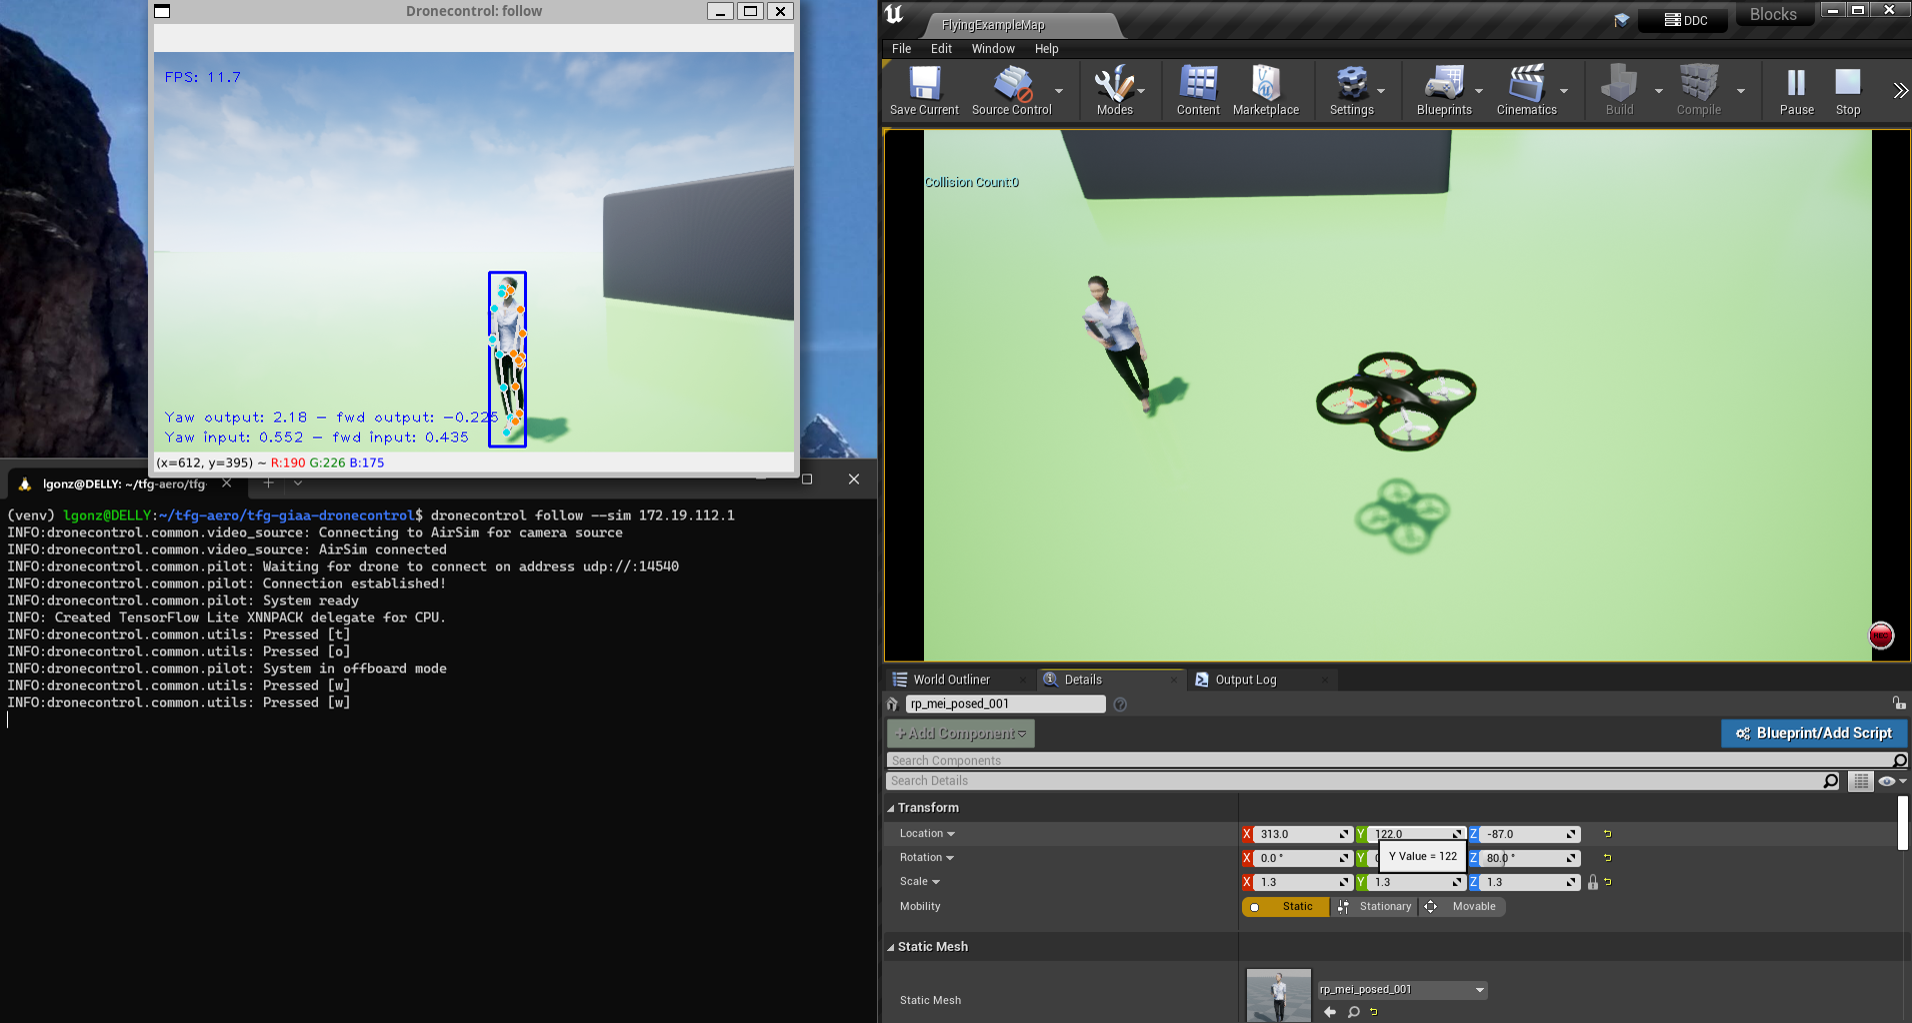
\includegraphics[width=\textwidth, keepaspectratio]{img/video-follow-sitl.png}
  \caption{Single frame from the video showing the movement of the drone in response to changes in the position of the tracked person}
  \label{fig:airsim-test-follow}
\end{figure}
